\documentclass[aspectratio=169,11pt]{beamer}

\usepackage[utf8]{inputenc}
\usepackage[T1]{fontenc}
\usepackage[turkish]{babel}
\usepackage{amsmath,amssymb}
\usepackage{graphicx}
\usepackage{booktabs}
\usepackage{tikz}
\usetikzlibrary{shapes.geometric,arrows.meta,positioning,calc}

% ---- Tema ve Renk ----
\usetheme{Madrid}
\usecolortheme{seahorse}
\setbeamertemplate{navigation symbols}{}
\setbeamertemplate{footline}[frame number]

\definecolor{cRemote}{HTML}{4E79A7}
\definecolor{cContext}{HTML}{F28E2B}
\definecolor{cInsitu}{HTML}{E15759}
\definecolor{cChem}{HTML}{76B7B2}
\definecolor{cContam}{HTML}{59A14F}
\definecolor{cFusion}{HTML}{EDC948}
\definecolor{cLow}{HTML}{D62728}
\definecolor{cHigh}{HTML}{2CA02C}
\definecolor{cExtra}{HTML}{9467BD}
\definecolor{bgDark}{HTML}{1B2838}

\setbeamercolor{title}{fg=white,bg=bgDark}
\setbeamercolor{frametitle}{fg=white,bg=cRemote}
\setbeamercolor{block title}{fg=white,bg=cRemote}
\setbeamercolor{block body}{bg=cRemote!8}
\setbeamercolor{item}{fg=cRemote}

\graphicspath{{img/}}

\title[Biyo-iz Güven Skoru]{Derin Uzay Astrobiyolojisi İçin\\Biyo-iz Güven Skoru}
\subtitle{Uzaktan Algılamadan Yakın Doğrulamaya Çok Modlu Karar Modeli}
\author{Sercan Demirhan \and Gizem Demirhan}
\date{2026}
\institute{}

% =====================================================================
\begin{document}
\shorthandoff{=}

% ===== SLAYT 1: KAPAK =====
{
\setbeamercolor{background canvas}{bg=bgDark}
\begin{frame}[plain]
\vfill
\begin{center}
{\color{cFusion}\rule{0.6\textwidth}{1pt}}\\[10pt]
{\Huge\bfseries\color{white}Biyo-iz Güven Skoru}\\[6pt]
{\large\color{cFusion}Derin Uzay Astrobiyolojisi İçin Çok Modlu Karar Modeli}\\[18pt]
{\color{gray!60}\small Sercan Demirhan\quad$\cdot$\quad Gizem Demirhan}\\[8pt]
{\color{gray!50}\footnotesize 2026}\\[12pt]
{\color{cFusion}\rule{0.6\textwidth}{1pt}}
\end{center}
\vfill
\end{frame}
}

% ===== SLAYT 2: PROBLEM =====
\begin{frame}{Problem: Tek Kanal Neden Yetersiz?}

\begin{columns}[T]
\begin{column}{0.52\textwidth}
\begin{block}{Abiyotik Taklit Riski}
\begin{itemize}
  \item Stromatolit benzeri yapılar \(\neq\) biyolojik kanıt
  \item Evaporitik kristaller morfolojiyi taklit eder
  \item Fischer--Tropsch sentezi organik molekül üretir
  \item \textbf{Tek kanala güvenmek \(\rightarrow\) yanlış pozitif}
\end{itemize}
\end{block}

\vspace{6pt}
\begin{alertblock}{Sonuç}
  Güvenilir yorum için \textbf{çoklu kanıt birleştirmesi} şarttır.
\end{alertblock}
\end{column}

\begin{column}{0.45\textwidth}
\centering
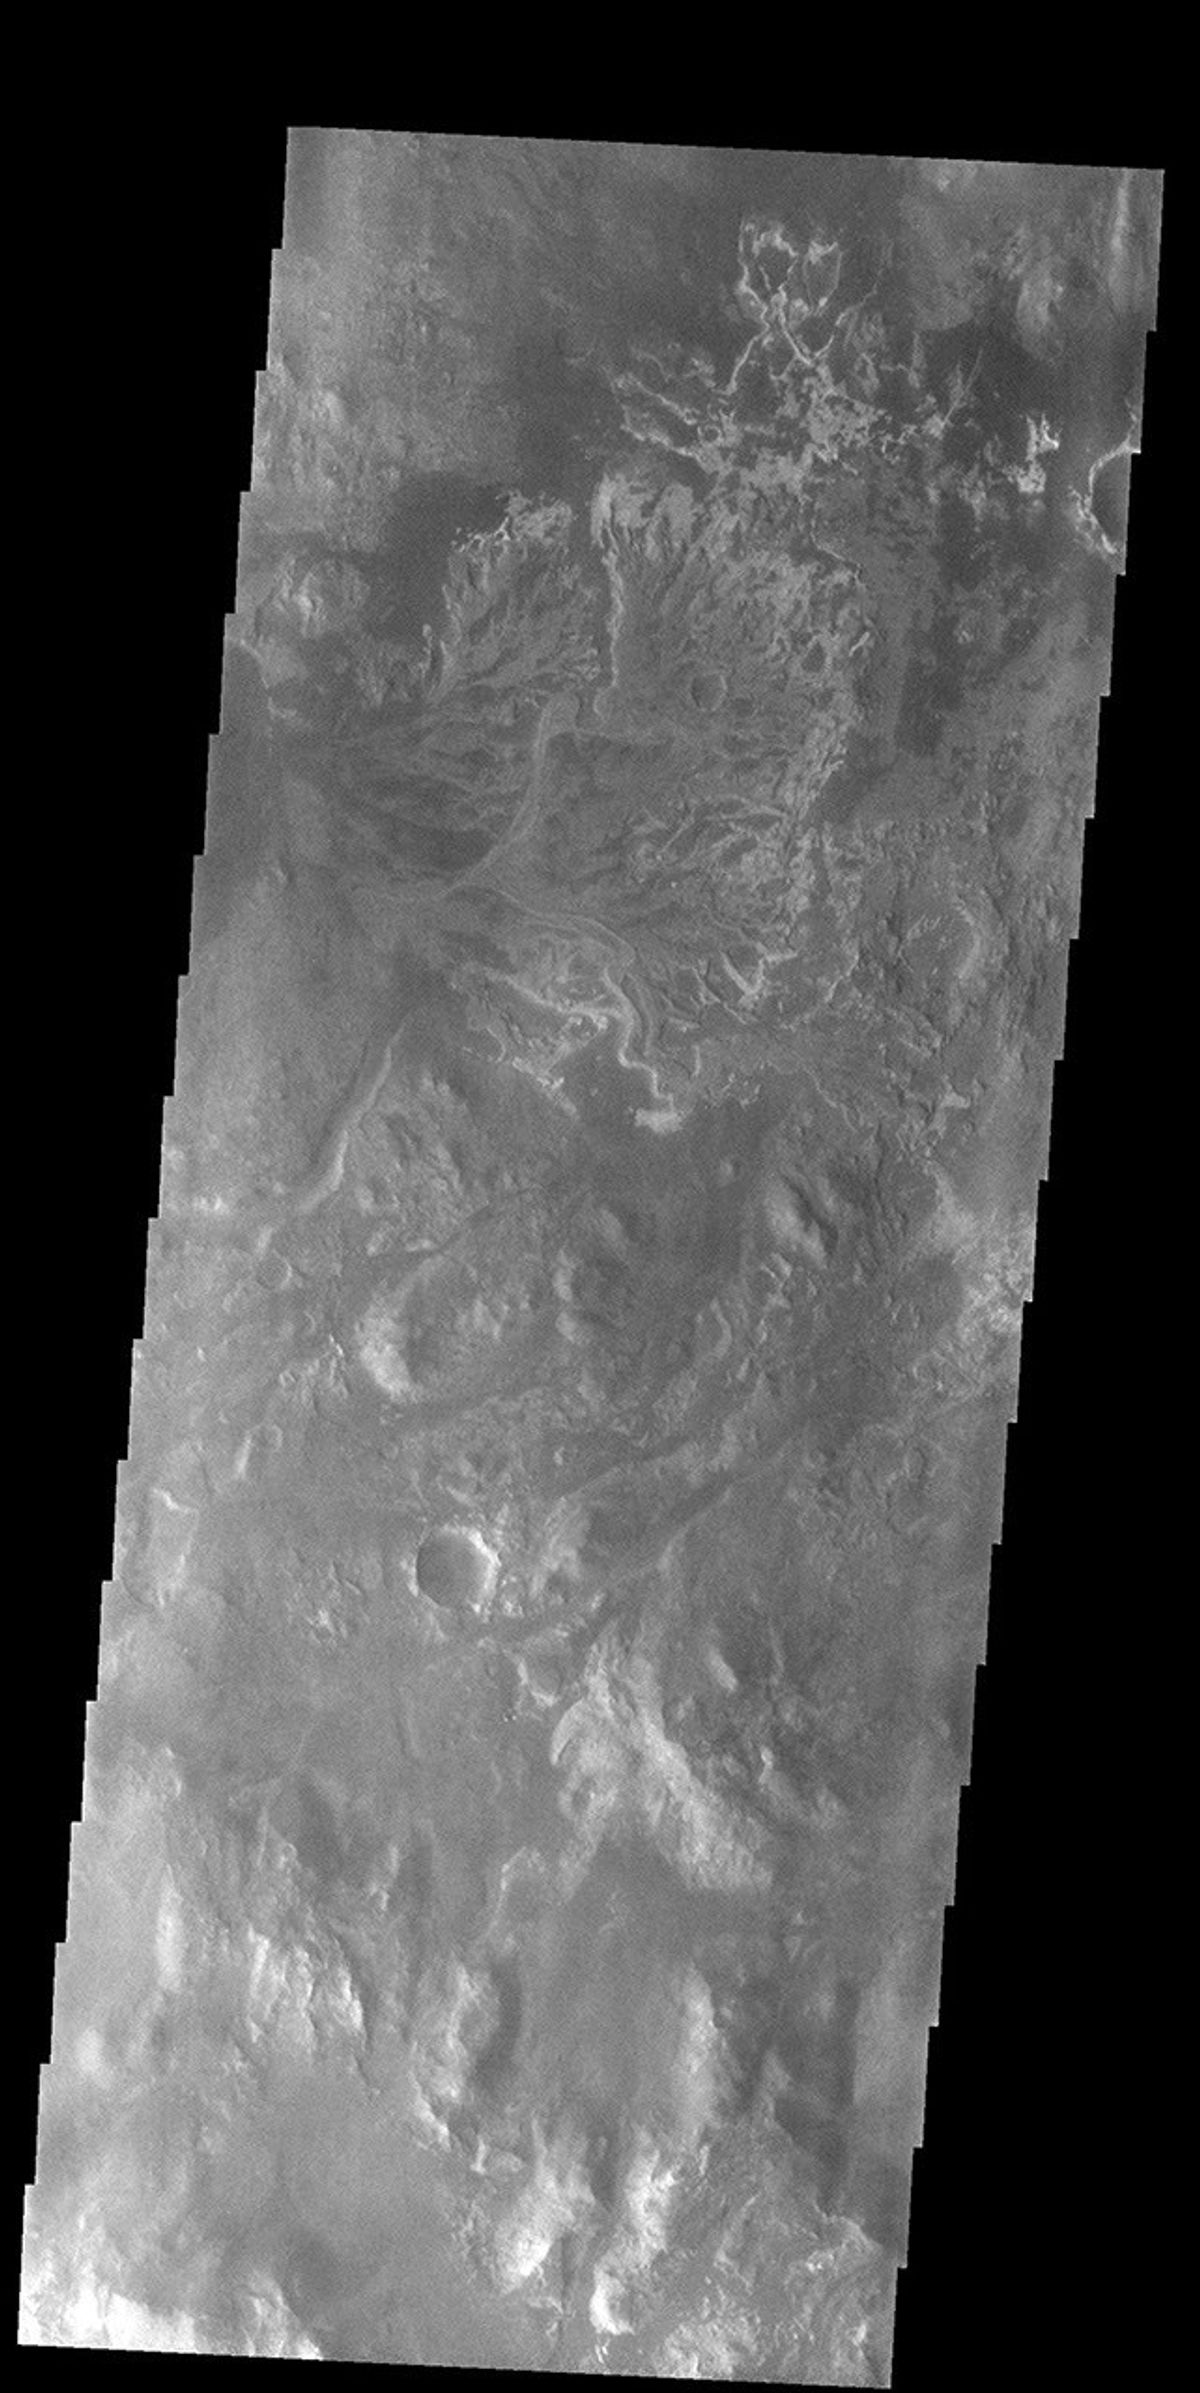
\includegraphics[width=\linewidth]{mars_rocks_closeup.jpg}\\[2pt]
{\tiny\color{gray} Mars kaya yüzeyi detayı --- NASA/JPL-Caltech (PIA25543)}
\end{column}
\end{columns}

\end{frame}

% ===== SLAYT 3: ÇÖZÜM — 5 Kanallı Bayes Modeli =====
\begin{frame}{Çözüm: 5 Kanallı Bayes Karar Modeli}

\begin{center}
\begin{tikzpicture}[
    node distance=0.55cm and 0.25cm,
    chan/.style={rectangle, draw, rounded corners=3pt, minimum width=2.3cm, minimum height=0.7cm, font=\scriptsize\bfseries, text=white, align=center},
    fuse/.style={rectangle, draw, rounded corners=3pt, minimum width=4.2cm, minimum height=0.7cm, font=\scriptsize\bfseries, fill=cFusion, text=black, align=center},
    arr/.style={-{Stealth[length=2mm]}, thick}
]
\node[chan, fill=cRemote]  (c1) {Uzaktan Tarama\\$S_{remote}$};
\node[chan, fill=cContext, right=of c1] (c2) {Jeolojik Bağlam\\$S_{context}$};
\node[chan, fill=cInsitu, right=of c2]  (c3) {Morfoloji\\$S_{in\text{-}situ}$};
\node[chan, fill=cChem, right=of c3]    (c4) {Kimya-İzotop\\$S_{chem\text{-}iso}$};
\node[chan, fill=cContam, right=of c4]  (c5) {Kontaminasyon\\$-\lambda R_{contam}$};

\node[fuse, below=0.8cm of c3] (fusion) {Bayes Füzyon $\rightarrow$ $S_{final}$};

\foreach \n in {c1,c2,c3,c4,c5} {
  \draw[arr] (\n.south) -- (fusion);
}
\end{tikzpicture}
\end{center}

\vspace{2pt}
\begin{equation*}
S_{final} = \alpha\, S_{remote} + \beta\, S_{context} + \gamma\, S_{in\text{-}situ} + \delta\, S_{chem\text{-}iso} - \lambda\, R_{contam}
\end{equation*}

\vspace{-4pt}
{\small
\begin{itemize}
  \item Her yeni ölçüm paketi $\rightarrow$ Bayes güncelleme ile sonsal olasılık artar/azalır
  \item Abiyotik açıklama güçlüyse skor \textbf{otomatik düşer}
  \item Karar etiketleri: \textcolor{cLow}{\textbf{Düşük}} $<0{,}35$ ~|~ \textcolor{cExtra}{\textbf{Ek Ölçüm}} ~|~ \textcolor{cHigh!70!black}{\textbf{Orta}} ~|~ \textcolor{cHigh}{\textbf{Yüksek}} $\geq0{,}80$
\end{itemize}
}

\end{frame}

% ===== SLAYT 4: DÜNYA ANALOGLARI =====
\begin{frame}{Dünya Analogları: Zemin Doğruluğu}

\begin{columns}[T]
\begin{column}{0.48\textwidth}
\centering
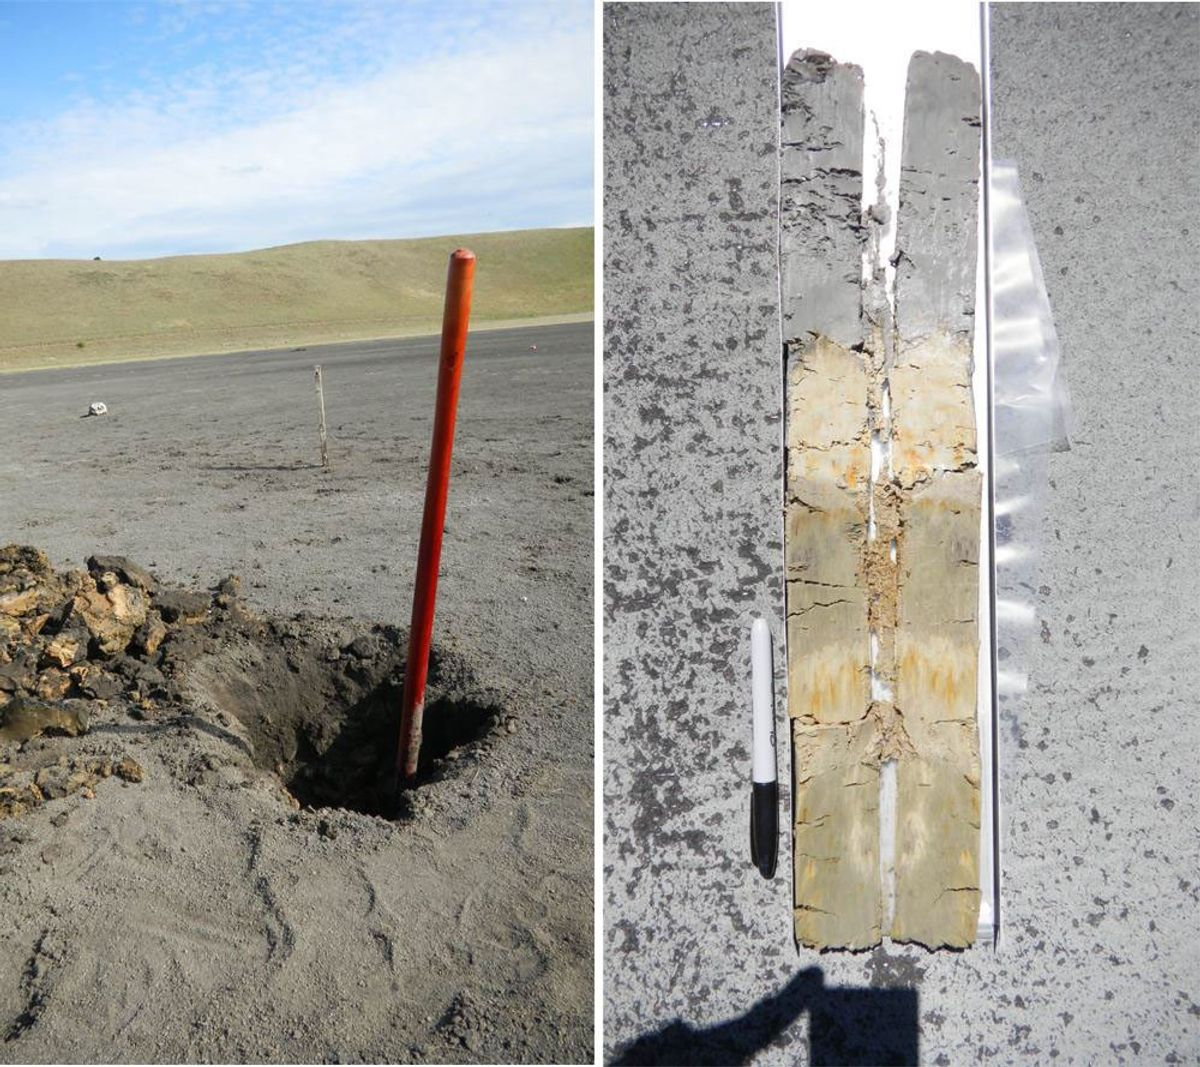
\includegraphics[width=\linewidth]{earth_analog.jpg}\\[2pt]
{\tiny\color{gray} Mars Yellowknife Bay Dünya analoğu --- NASA/JPL-Caltech (PIA16831)}

\vspace{6pt}
\begin{block}{Neden Dünya Analogları?}
\begin{itemize}\small
  \item Bilinen biyotik imzalarla model kalibrasyonu
  \item Shark Bay stromatolitleri $\rightarrow$ \textbf{pozitif kontrol}
  \item Yellowstone sinter $\rightarrow$ \textbf{hidrotermal biyo-iz}
  \item Evaporit/demir oksit $\rightarrow$ \textbf{negatif kontrol}
\end{itemize}
\end{block}
\end{column}

\begin{column}{0.48\textwidth}
\centering
\small
\begin{tabular}{lcc}
\toprule
\textbf{Senaryo} & $S_{final}$ & \textbf{Etiket}\\
\midrule
Shark Bay      & 0{,}91 & \textcolor{cHigh}{Yüksek}\\
Yellowstone    & 0{,}84 & \textcolor{cHigh}{Yüksek}\\
Arsenik mat    & 0{,}73 & Orta\\
\midrule
Death Valley   & 0{,}31 & \textcolor{cLow}{Düşük}\\
Demir oksit    & 0{,}22 & \textcolor{cLow}{Düşük}\\
Fischer--Tropsch & 0{,}28 & \textcolor{cLow}{Düşük}\\
\bottomrule
\end{tabular}

\vspace{10pt}
\textbf{12/12 doğru karar} --- Karışıklık matrisinde sıfır yanlış pozitif
\end{column}
\end{columns}

\end{frame}

% ===== SLAYT 5: MARS ANALİZİ =====
\begin{frame}{Mars Analizi: Jezero Krateri ve Perseverance Verileri}

\begin{columns}[T]
\begin{column}{0.48\textwidth}
\centering
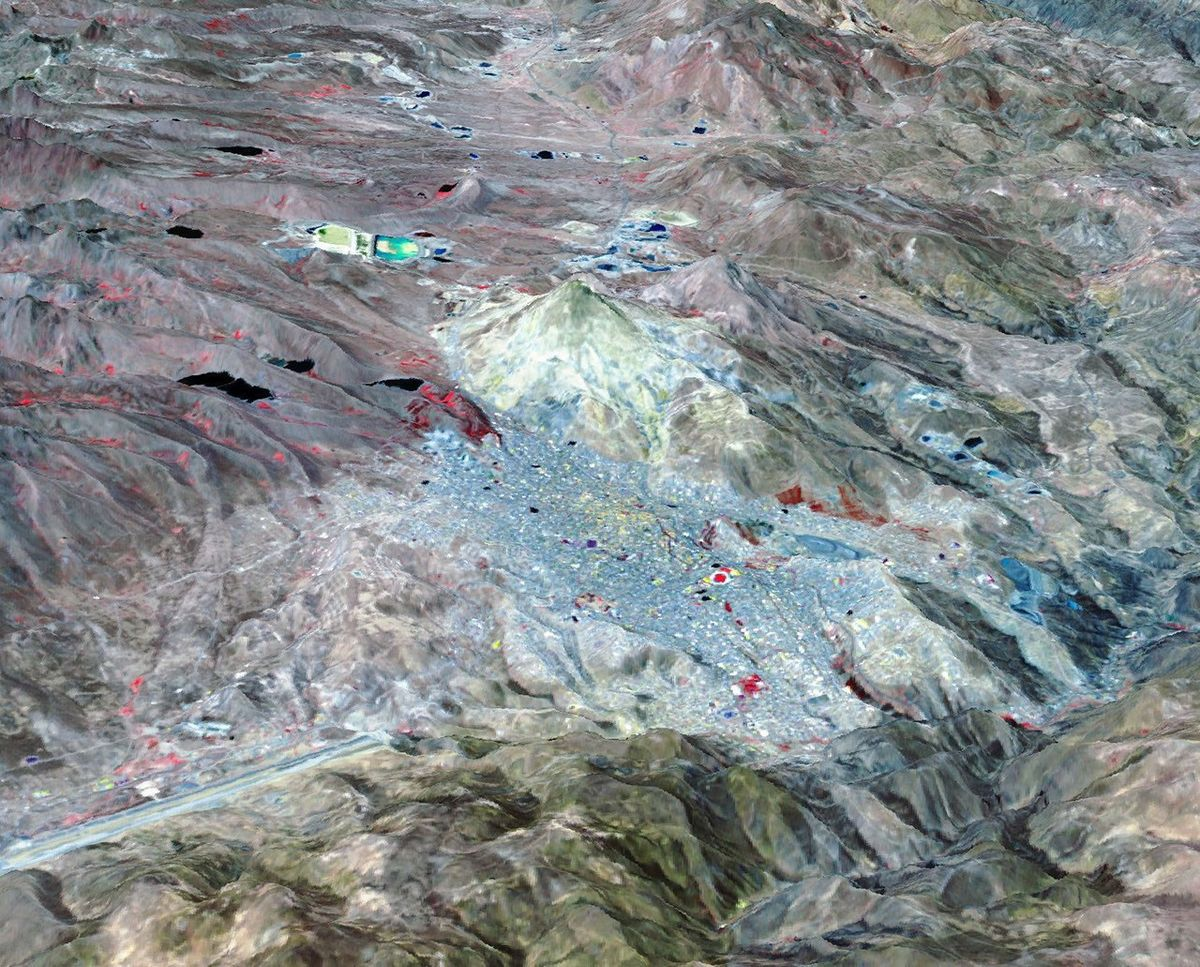
\includegraphics[width=\linewidth]{mars_jezero_delta.jpg}\\[2pt]
{\tiny\color{gray} Jezero Krateri deltası --- NASA/JPL-Caltech (PIA25705)}

\vspace{4pt}
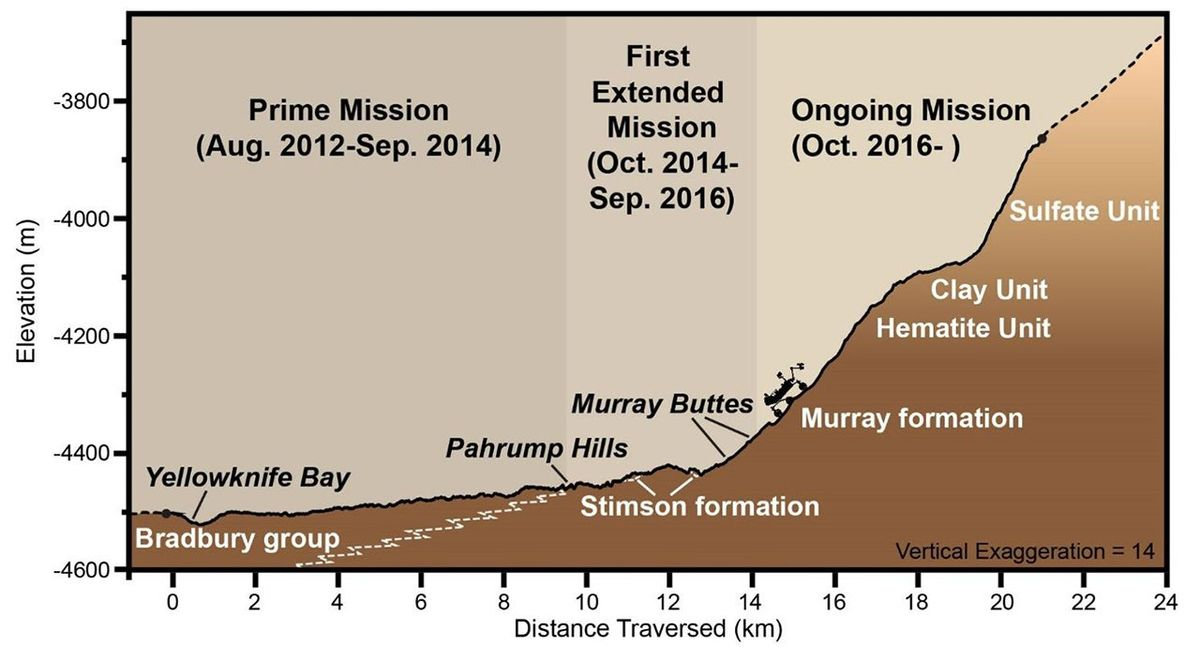
\includegraphics[width=0.75\linewidth]{mars_hirise_layers.jpg}\\[2pt]
{\tiny\color{gray} HiRISE sedimanter katmanlar (PIA21145)}
\end{column}

\begin{column}{0.48\textwidth}
\begin{block}{Kullanılan Veri Kaynakları}
\begin{itemize}\small
  \item \textbf{CRISM}: VNIR-SWIR mineral haritası
  \item \textbf{HiRISE}: yüksek çözünürlük morfoloji
  \item \textbf{PIXL}: XRF element dağılımı
  \item \textbf{SHERLOC}: Raman + floresans
  \item \textbf{SuperCam}: LIBS spektroskopi
\end{itemize}
\end{block}

\vspace{4pt}
\small
\begin{tabular}{lcc}
\toprule
\textbf{Mars Senaryosu} & $S_{final}$ & \textbf{Etiket}\\
\midrule
Jezero delta   & 0{,}68 & Orta\\
Sülfat damar   & 0{,}52 & Ek ölçüm\\
Bazalt         & 0{,}18 & \textcolor{cLow}{Düşük}\\
\bottomrule
\end{tabular}
\end{column}
\end{columns}

\end{frame}

% ===== SLAYT 6: İŞLEM HATTI & SONUÇLAR =====
\begin{frame}{İşlem Hattı ve Doğrulama Sonuçları}

\begin{columns}[T]
\begin{column}{0.52\textwidth}
\begin{center}
\begin{tikzpicture}[
    node distance=0.4cm,
    stp/.style={rectangle, draw, rounded corners=2pt, minimum width=3.6cm, minimum height=0.5cm, font=\tiny\bfseries, text=white, align=center},
    arr/.style={-{Stealth[length=1.5mm]}, thick, gray!70}
]
\node[stp, fill=cRemote]   (f0)  {Faz 0: Referans Kütüphanesi};
\node[stp, fill=cRemote!85, below=of f0]  (f1) {Faz 1: Uzaktan Tarama};
\node[stp, fill=cContext, below=of f1] (f2) {Faz 2: Jeolojik Bağlam};
\node[stp, fill=cInsitu, below=of f2]  (f3) {Faz 3: Morfoloji};
\node[stp, fill=cChem, below=of f3]    (f4) {Faz 4: Kimya-İzotop};
\node[stp, fill=cContam, below=of f4]  (f5) {Faz 5--6: Karar Füzyonu};
\node[stp, fill=cFusion, text=black, below=of f5]  (out) {$S_{final}$ + Karar Etiketi};

\foreach \a/\b in {f0/f1, f1/f2, f2/f3, f3/f4, f4/f5, f5/out} {
  \draw[arr] (\a) -- (\b);
}
\end{tikzpicture}
\end{center}
\end{column}

\begin{column}{0.45\textwidth}
\begin{block}{Doğrulama Özeti}
\begin{itemize}\small
  \item \textbf{12 referans senaryo} test edildi
  \item \textbf{12/12 doğru karar} (tam tutarlılık)
  \item Karışıklık matrisi: \textbf{0 yanlış pozitif}
  \item Monte Carlo: $\sigma \approx 0{,}03$ belirsizlik
\end{itemize}
\end{block}

\vspace{4pt}
\begin{block}{Teknik Altyapı}
\begin{itemize}\small
  \item Python işlem hattı (açık kaynak)
  \item NASA PDS + ESA PSA verileri
  \item USGS Spectral Library v7
  \item SDSS teleskop spektrumları
  \item Bayes güncelleme + karar ağacı
\end{itemize}
\end{block}
\end{column}
\end{columns}

\end{frame}

% ===== SLAYT 7: SONUÇ & YOL HARİTASI =====
{
\setbeamercolor{background canvas}{bg=bgDark}
\begin{frame}[plain]
\vfill
\begin{center}
{\color{cFusion}\rule{0.55\textwidth}{1pt}}\\[10pt]
{\Large\bfseries\color{white}Sonuç ve Yol Haritası}\\[14pt]

\begin{minipage}{0.82\textwidth}
\color{gray!80}
\begin{columns}[T]
\begin{column}{0.48\textwidth}
\textbf{\color{cFusion}Temel Katkılar}
\begin{itemize}\small\color{gray!90}
  \item 5 kanallı Bayes karar modeli
  \item Abiyotik taklit baskılama
  \item 12/12 doğrulama başarısı
  \item Açık kaynak Python pipeline
  \item Gerçek NASA/PDS verileri
\end{itemize}
\end{column}
\begin{column}{0.48\textwidth}
\textbf{\color{cFusion}90 Günlük MVP}
\begin{itemize}\small\color{gray!90}
  \item[\color{cRemote}\textbullet] Gün 1--30: Veri şeması + uzaktan tarama modeli
  \item[\color{cContext}\textbullet] Gün 31--60: Bağlam + morfoloji entegrasyonu
  \item[\color{cChem}\textbullet] Gün 61--90: Kimya-izotop füzyon + gösterge paneli
\end{itemize}
\end{column}
\end{columns}
\end{minipage}

\vspace{16pt}
{\color{cFusion}\rule{0.55\textwidth}{1pt}}\\[8pt]
{\small\color{gray!50} github.com/Farondis/astrobiology-biosignature-score}
\end{center}
\vfill
\end{frame}
}

\end{document}
